\documentclass[conference]{IEEEtran}
\IEEEoverridecommandlockouts
\usepackage{cite}
\usepackage{amsmath,amssymb,amsfonts}
\usepackage{algorithmic}
\usepackage{graphicx}
\usepackage{textcomp}
\usepackage{xcolor}
\usepackage{booktabs}
\def\BibTeX{{\rm B\kern-.05em{\sc i\kern-.025em b}\kern-.08em
    T\kern-.1667em\lower.7ex\hbox{E}\kern-.125emX}}
\begin{document}

\title{Benchmarking Shor's Order-Finding Algorithm on IBM Quantum Hardware: A Three-Tier Comparative Analysis}

\author{\IEEEauthorblockN{Gabil Gurbanov}
\IEEEauthorblockA{\textit{School of Information Technologies and Engineering} \\
\textit{ADA University}\\
Baku, Azerbaijan \\
ggurbanov12098@ada.edu.az}
}

\maketitle

\begin{abstract}
This paper presents a systematic benchmarking study of Shor's order-finding algorithm for the case $N=15$, $a=2$, executed across three distinct tiers: ideal (noiseless) simulation, noisy simulation with device-calibrated error models, and real IBM Quantum hardware. A total of 48 experimental configurations were evaluated on the 156-qubit ibm\_marrakesh processor, varying transpilation optimisation level (0--3), control-register precision (4, 6, 8 qubits), resilience level (0--1), and dynamical decoupling (on/off). Performance was quantified using Total Variation Distance and success probability metrics. The highest hardware success probability of 88.4\% was achieved with 4 control qubits at optimisation level 2, while 8-control-qubit configurations degraded to near-random output at low optimisation levels. These results quantify the gap between theoretical quantum algorithmic performance and practical hardware execution, providing empirical evidence for the impact of transpilation optimisation and error mitigation on circuit fidelity.
\end{abstract}

\begin{IEEEkeywords}
quantum computing, Shor's algorithm, quantum benchmarking, IBM Quantum, Qiskit, error mitigation, order finding
\end{IEEEkeywords}

\section{Introduction}

Quantum computing promises exponential speedups for specific computational problems that remain intractable for classical machines. Among the most consequential quantum algorithms is Shor's algorithm~\cite{b1}, which factors large integers in polynomial time by reducing the factorisation problem to order finding via quantum phase estimation. The theoretical implications of this algorithm for public-key cryptography, particularly RSA, have motivated substantial research into both quantum hardware development and post-quantum cryptographic alternatives~\cite{b2}.

Despite the theoretical elegance of Shor's algorithm, practical execution on current noisy intermediate-scale quantum (NISQ) devices remains challenging. Hardware noise, limited qubit coherence times, gate errors, and connectivity constraints introduce significant fidelity degradation~\cite{b3}. Quantifying this gap between ideal algorithmic behaviour and real hardware performance is essential for assessing the current state of quantum computing and guiding future hardware and software improvements.

This work addresses the following research objective: to systematically benchmark Shor's order-finding algorithm on real IBM Quantum hardware by comparing ideal simulation, noisy simulation, and hardware execution across a comprehensive set of configurations. The study employs a full factorial experimental design spanning transpilation optimisation levels, control-register sizes, error mitigation settings, and dynamical decoupling, yielding 48 distinct experimental configurations executed on the \texttt{ibm\_marrakesh} backend.

\subsection{Abbreviations and Acronyms}
The following abbreviations are used throughout this paper:
\begin{itemize}
\item \textbf{NISQ} --- Noisy Intermediate-Scale Quantum
\item \textbf{QFT} --- Quantum Fourier Transform
\item \textbf{QPE} --- Quantum Phase Estimation
\item \textbf{TVD} --- Total Variation Distance
\item \textbf{DD} --- Dynamical Decoupling
\item \textbf{RSA} --- Rivest--Shamir--Adleman cryptosystem
\item \textbf{2Q} --- Two-Qubit (gate)
\item \textbf{QC} --- Quantum Computing
\item \textbf{SDK} --- Software Development Kit
\end{itemize}

\section{Related Work}

Prior work has established the theoretical foundations and early experimental demonstrations of Shor's algorithm. Bhatia and Ramkumar~\cite{b1} demonstrated an efficient quantum computing technique for cryptanalysis using Shor's algorithm, highlighting its potential to compromise RSA encryption. Lanyon et al.~\cite{b4} reported photonic implementations of Shor's algorithm, demonstrating factorisation on small-scale quantum systems with limited qubit counts.

The architectural evolution of quantum computing frameworks has been examined by Ahmad, Earnest-Noble, and Byrd~\cite{b5}, who explored the Qiskit Runtime architecture for educational and research enablement, demonstrating the accessibility of IBM's quantum cloud infrastructure for algorithm development and execution. Comparative analyses of quantum frameworks, including Qiskit and Cirq, have shown that Qiskit's transpiler design and error mitigation capabilities offer advantages for hardware execution, particularly when circuit depth optimisation is combined with runtime error mitigation techniques~\cite{b5}.

The broader implications of quantum computing for cryptographic security have been extensively studied. Bernstein and Lange~\cite{b2} provided a comprehensive survey of post-quantum cryptography, identifying lattice-based, code-based, and hash-based schemes as promising quantum-resistant candidates. Mahmoud~\cite{b6} examined the role of quantum computing in the cybersecurity landscape, emphasising the urgency of deploying quantum-resistant cryptographic standards. Kumar et al.~\cite{b7} investigated implementations of both Grover's and Shor's algorithms in quantum machine learning contexts. Prior work by Gurbanov~\cite{b8} provided a detailed analysis of quantum threats to cryptographic systems, covering both Shor's and Grover's algorithms alongside post-quantum mitigation strategies, laying the groundwork for the present experimental investigation.

\section{Methodology}

\subsection{Circuit Construction}

The quantum circuit implements Shor's order-finding subroutine for $N=15$, $a=2$, where the true order is $r=4$. The circuit comprises two registers: a variable-size control register ($t \in \{4, 6, 8\}$ qubits) for phase estimation and a 4-qubit target register for modular arithmetic, yielding total circuit sizes of 8, 10, and 12 qubits respectively.

The target register is initialised to $|1\rangle$. For each control qubit $k$, a Hadamard gate creates superposition, followed by a controlled modular multiplication gate implementing $a^{2^k} \bmod N$. The modular gates are constructed as follows: $M_2 \bmod 15$ is realised via three SWAP gates implementing a cyclic left-shift, while $M_4 \bmod 15$ uses two SWAP gates for a pair-wise swap. When $a^{2^k} \bmod N = 1$, the corresponding gate reduces to identity and is omitted. The inverse Quantum Fourier Transform (QFT) is applied to the control register, followed by measurement of all control qubits.

\subsection{Three-Tier Execution Framework}

Three execution tiers provide complementary perspectives on algorithm performance:

\textbf{Tier A --- Ideal Simulation.} Noiseless execution via Qiskit's \texttt{StatevectorSampler} with 100,000 shots establishes the theoretical baseline, producing success probability of 1.0 for all configurations.

\textbf{Tier B --- Noisy Simulation.} The Qiskit Aer \texttt{AerSimulator} with a noise model derived from the \texttt{ibm\_marrakesh} backend calibration data provides an intermediate reference. When device-calibrated models are unavailable, a generic depolarising model is employed (0.1\% single-qubit error, 1\% two-qubit error).

\textbf{Tier C --- Real Hardware.} Circuits are executed on IBM's 156-qubit \texttt{ibm\_marrakesh} processor via the Qiskit Runtime \texttt{SamplerV2} primitive with 1,024 shots per configuration.

\subsection{Performance Metrics}

Two metrics quantify execution quality. The \textit{Total Variation Distance} (TVD) between distributions $P$ and $Q$ is defined as:
\begin{equation}
\text{TVD}(P, Q) = \frac{1}{2} \sum_{x} |P(x) - Q(x)|
\label{eq:tvd}
\end{equation}
where values range from 0 (identical) to 1 (completely disjoint). Three TVD variants are computed: hardware vs.\ ideal, hardware vs.\ noisy, and noisy vs.\ ideal.

The \textit{success probability} measures the total probability mass falling within an $\varepsilon$-window of expected Shor peaks. For $a=2$, $N=15$, the expected phases are $\theta_k \in \{0, 0.25, 0.5, 0.75\}$, with tolerance $\varepsilon = 1/2^{t+1}$ scaling with phase-estimation precision.

\section{Experimental Setup}

\subsection{Sweep Parameters}

A full factorial design was employed across four axes: transpilation optimisation level $\in \{0, 1, 2, 3\}$, control-qubit count $\in \{4, 6, 8\}$, resilience level $\in \{0, 1\}$, and dynamical decoupling (XpXm sequence) $\in \{\text{off}, \text{on}\}$, producing $4 \times 3 \times 2 \times 2 = 48$ configurations. Each configuration was executed across all three tiers with a fixed transpiler seed of 42 for reproducibility.

\subsection{Transpilation and Error Mitigation}

Qiskit's \texttt{generate\_preset\_pass\_manager} compiled circuits to the native gate set of the target backend. Resilience level 1 activates twirling-based readout error mitigation, while dynamical decoupling inserts XpXm pulse sequences during idle periods to suppress decoherence. Gate twirling was enabled for all hardware executions.

\section{Results and Analysis}

\subsection{Transpilation Impact on Circuit Depth}

Table~\ref{tab:depth} summarises the two-qubit gate depth and count after transpilation. Higher optimisation levels consistently reduced circuit complexity, with the most substantial reduction occurring between levels 0 and 2.

\begin{table}[htbp]
\caption{Transpiled Circuit Metrics by Control-Qubit Count and Optimisation Level}
\begin{center}
\begin{tabular}{cccc}
\toprule
\textbf{Ctrl Qubits} & \textbf{Opt Level} & \textbf{2Q Depth} & \textbf{2Q Count} \\
\midrule
4 & 0 & 218 & 249 \\
4 & 1 & 188 & 198 \\
4 & 2 & 155 & 164 \\
4 & 3 & 155 & 164 \\
\midrule
6 & 0 & 284 & 363 \\
6 & 1 & 212 & 252 \\
6 & 2 & 181 & 209 \\
6 & 3 & 181 & 209 \\
\midrule
8 & 0 & 366 & 560 \\
8 & 1 & 270 & 350 \\
8 & 2 & 193 & 263 \\
8 & 3 & 190 & 274 \\
\bottomrule
\end{tabular}
\label{tab:depth}
\end{center}
\end{table}

\subsection{Hardware Success Probability}

The ideal simulation achieved a success probability of 1.0 across all configurations. The noisy simulation produced success probabilities of 0.946, 0.883, and 0.856 for 4, 6, and 8 control qubits respectively, reflecting the increasing circuit depth.

On real hardware, the best result was a success probability of 0.884 (4 control qubits, optimisation level 2, resilience 0, dynamical decoupling off), with a corresponding TVD of 0.155 against the ideal distribution. The worst hardware result was 0.023 (8 control qubits, optimisation level 0, resilience 0, dynamical decoupling off), with TVD of 0.977, indicating near-random output.

For the 4-control-qubit configurations, optimisation levels 2 and 3 consistently yielded hardware success probabilities above 0.77, while level 0 without dynamical decoupling dropped to 0.397. The 6-control-qubit circuits achieved a maximum hardware success probability of 0.673 at optimisation level 3 with resilience 1. The 8-control-qubit circuits demonstrated severe fidelity degradation, with the best configuration reaching only 0.449 at optimisation level 3 with resilience 1.

Fig.~\ref{fig:sptvd} presents the success probability and TVD trends across optimisation levels, grouped by control-qubit count. A clear inverse relationship is observed: as optimisation level increases, success probability rises while TVD decreases, with the effect most pronounced for 4-control-qubit circuits.

\begin{figure}[htbp]
\centerline{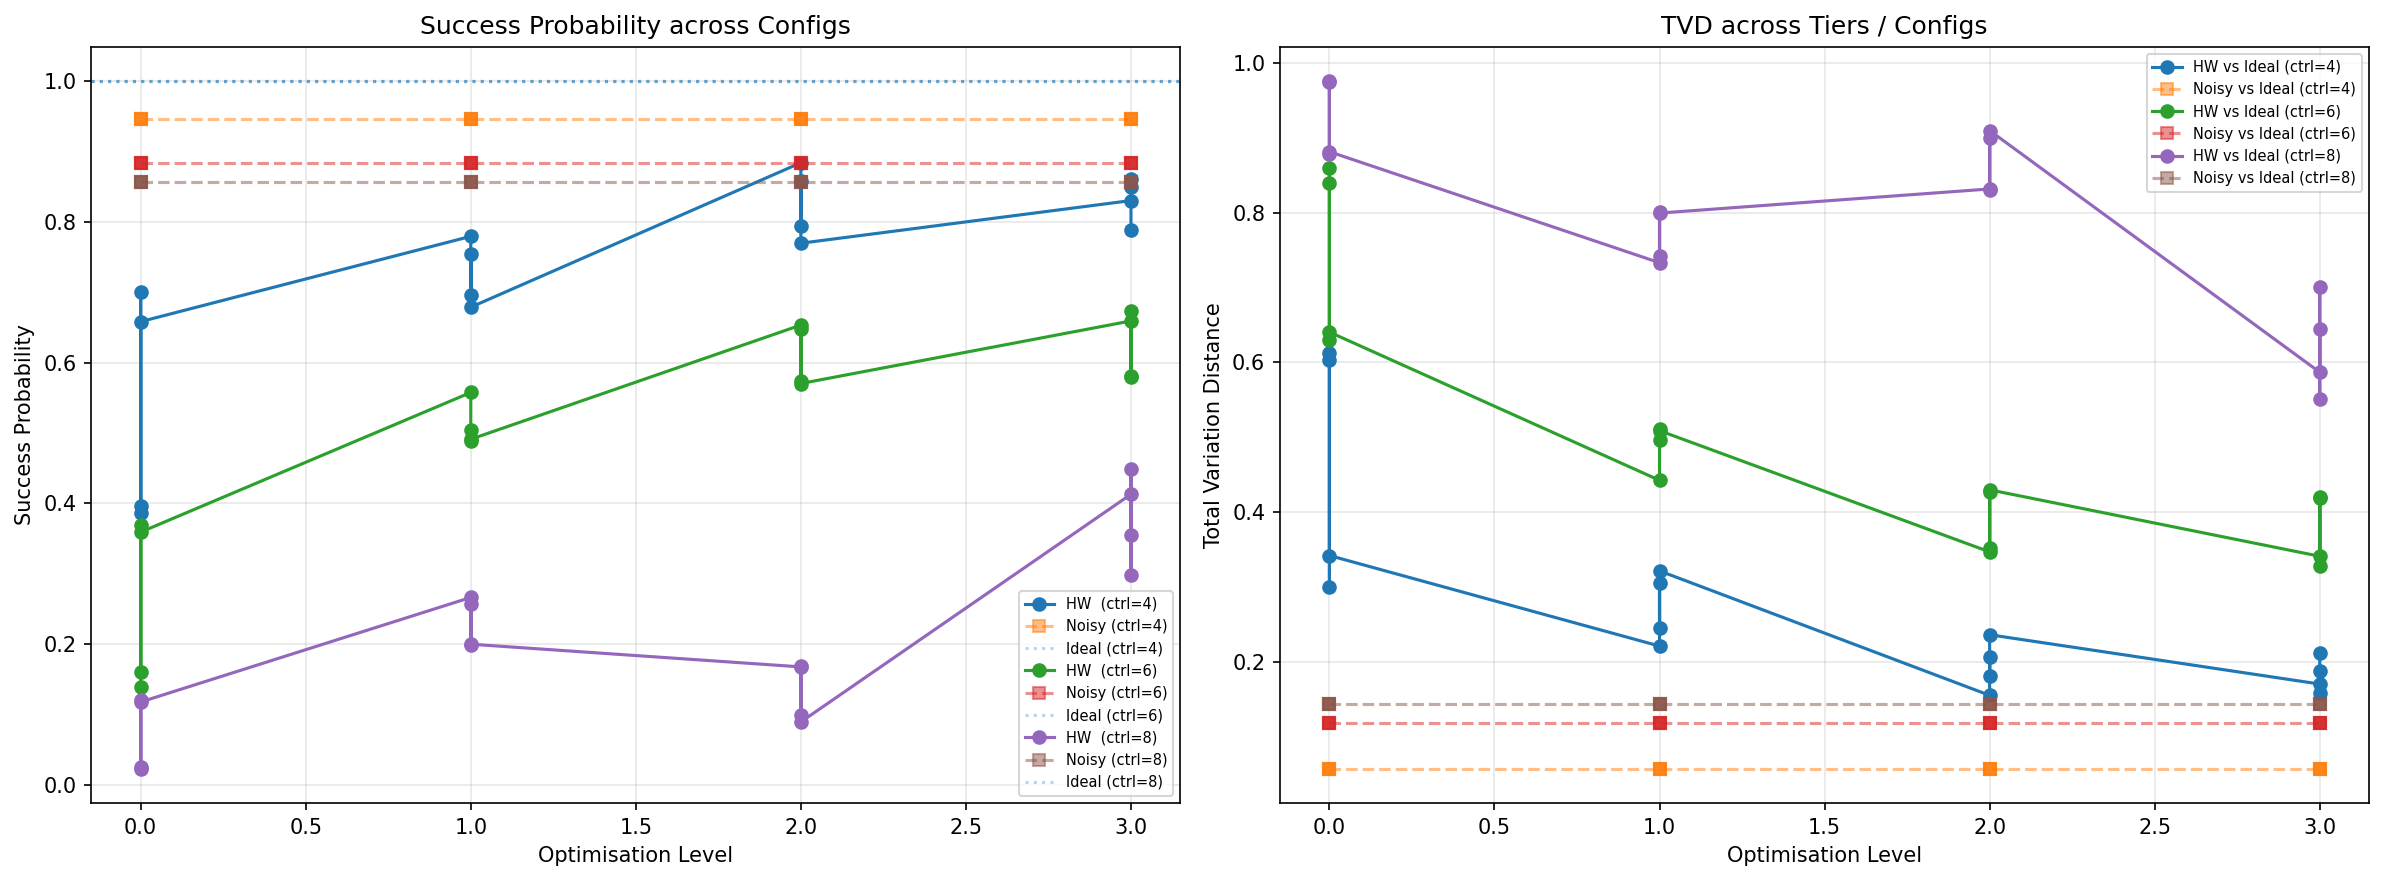
\includegraphics[width=\columnwidth]{success_prob_and_tvd.png}}
\caption{Success probability (left) and Total Variation Distance (right) across transpilation optimisation levels for 4, 6, and 8 control qubits. Higher optimisation levels consistently improve fidelity, with diminishing returns between levels 2 and 3.}
\label{fig:sptvd}
\end{figure}

Fig.~\ref{fig:bar} provides a grouped bar chart comparing Ideal, Noisy, and Hardware success probabilities for all 48 configurations. The progressive degradation from ideal to noisy to hardware is visible across all settings, with the gap widening substantially for deeper circuits.

\begin{figure}[htbp]
\centerline{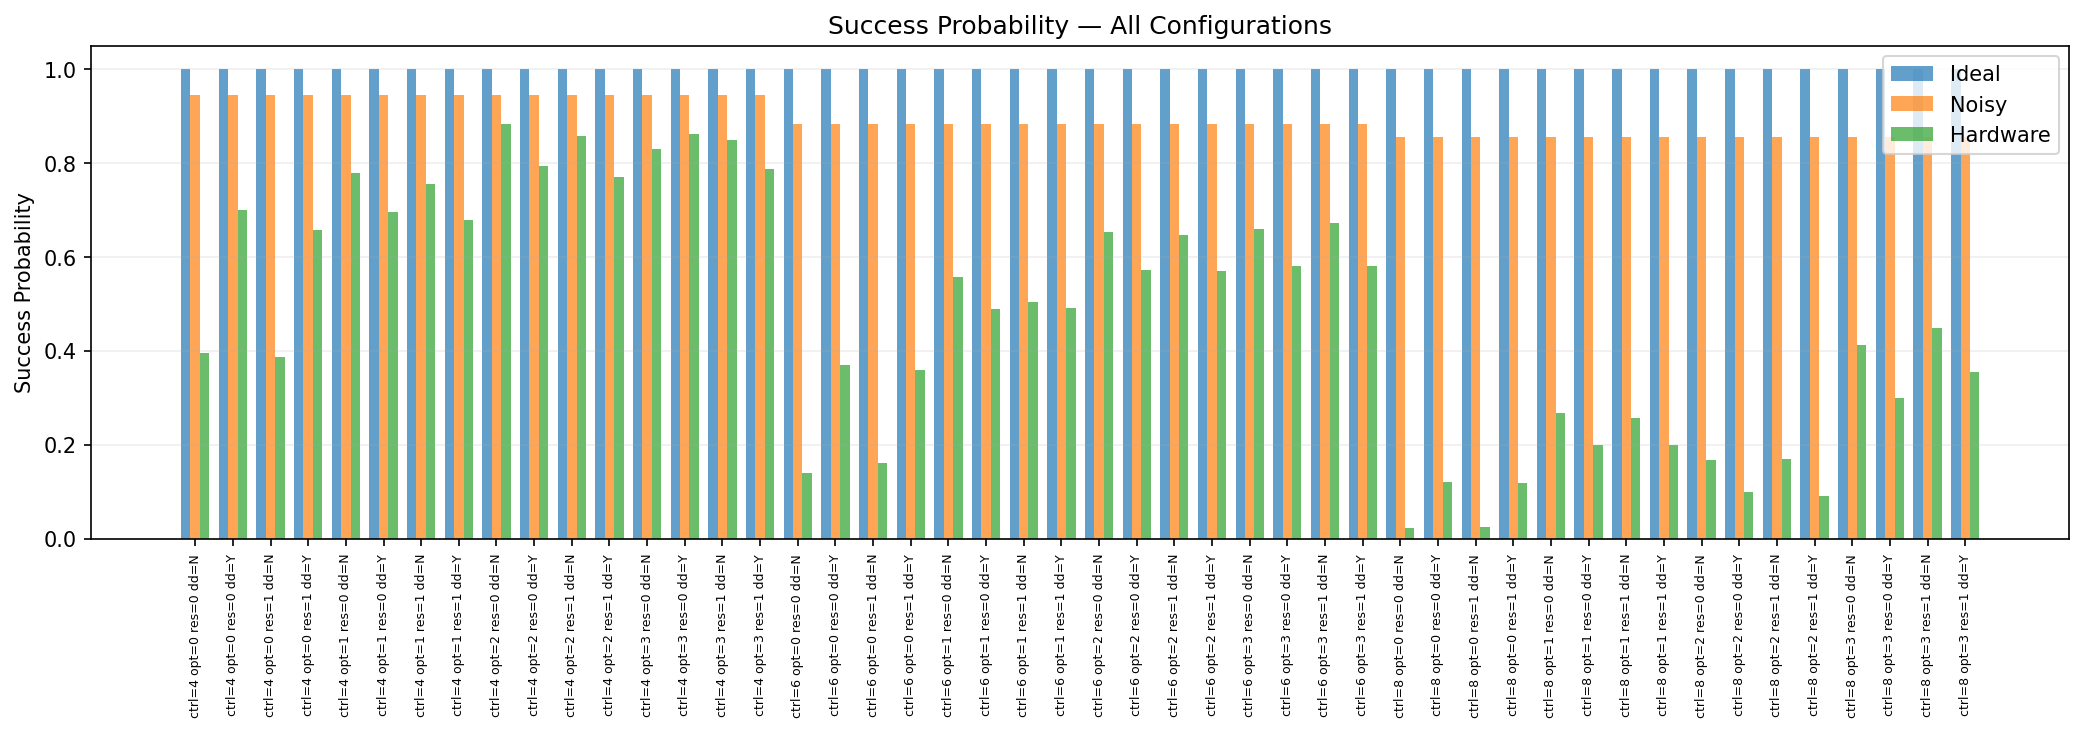
\includegraphics[width=\columnwidth]{success_prob_bar.png}}
\caption{Grouped bar chart of success probability across all 48 experimental configurations, comparing Ideal (Tier A), Noisy (Tier B), and Hardware (Tier C) execution. Each group represents a unique combination of control qubits, optimisation level, resilience level, and DD setting.}
\label{fig:bar}
\end{figure}

\subsection{Effect of Error Mitigation Techniques}

Dynamical decoupling exhibited configuration-dependent behaviour. At optimisation level 0 with 4 control qubits, enabling dynamical decoupling increased success probability from 0.397 to 0.700---a 76\% relative improvement. However, at higher optimisation levels where circuit idle periods are already minimised, dynamical decoupling occasionally reduced performance. Resilience level 1 provided marginal improvements in most 4-control-qubit configurations but did not consistently outperform the baseline across all settings.

\section{Discussion}

The experimental results demonstrate a clear hierarchy of factors influencing hardware fidelity. Transpilation optimisation level has the most significant impact, reducing two-qubit gate depth by up to 29\% (from 218 to 155 for 4 control qubits) and substantially improving success probability. The precision--noise trade-off is evident: increasing control qubits from 4 to 8 improves theoretical phase resolution from $1/16$ to $1/256$ but increases circuit depth to the point where decoherence overwhelms the precision advantage.

The noisy simulation provides a useful but imperfect predictor of hardware behaviour. The TVD between hardware and noisy simulation (0.127--0.870 across configurations) indicates that device-calibrated noise models capture bulk error characteristics but fail to account for all sources of hardware imperfection, such as crosstalk, drift, and non-Markovian effects.

A key limitation of this study is the restriction to $N=15$, the smallest non-trivial case for Shor's algorithm. While this enables feasible execution on current hardware, the results may not generalise to larger factorisations requiring significantly deeper circuits and more qubits. Additionally, all experiments were conducted on a single backend (\texttt{ibm\_marrakesh}) during a single session, and performance may vary across different devices and calibration cycles.

\section{Conclusion and Future Work}

This study provides a comprehensive empirical characterisation of Shor's order-finding algorithm on IBM Quantum hardware, demonstrating that transpilation optimisation and circuit depth are the dominant factors in determining execution fidelity. The best hardware configuration achieved 88.4\% success probability with a TVD of 0.155 against ideal, while deeper circuits with 8 control qubits degraded to near-random output at low optimisation levels.

Future work will extend this benchmarking framework to larger values of $N$, evaluate additional error mitigation strategies including zero-noise extrapolation, and perform cross-backend comparisons across multiple IBM Quantum processors. Factor extraction via continued fractions from hardware measurement distributions will be further validated and analysed. Further experimental validation of advanced error mitigation techniques on newer quantum hardware generations is ongoing.

\begin{thebibliography}{00}
\bibitem{b1} V. Bhatia and K. R. Ramkumar, ``An efficient quantum computing technique for cracking RSA using Shor's algorithm,'' in \textit{Proc. IEEE 5th Int. Conf. Computing Communication and Automation (ICCCA)}, Greater Noida, India, 2020, pp. 89--94, doi: 10.1109/ICCCA49541.2020.9250806.
\bibitem{b2} D. J. Bernstein and T. Lange, ``Post-quantum cryptography,'' \textit{Nature}, vol. 549, no. 7671, pp. 188--194, 2017, doi: 10.1038/nature23461.
\bibitem{b3} D. Rosch-Grace and J. Straub, ``Considering the implications of artificial intelligence, quantum computing, and cybersecurity,'' in \textit{Proc. 2022 Int. Conf. Computational Science and Computational Intelligence (CSCI)}, Las Vegas, NV, USA, Dec. 2022, pp. 1080--1083, doi: 10.1109/CSCI58124.2022.00191.
\bibitem{b4} B. P. Lanyon \textit{et al.}, ``Photonic quantum computing: Shor's algorithm and the road to fault-tolerance,'' in \textit{2008 Conf. Lasers and Electro-Optics and 2008 Conf. Quantum Electronics and Laser Science}, San Jose, CA, USA, 2008, pp. 1--2.
\bibitem{b5} S. F. Ahmad, N. Earnest-Noble, and G. T. Byrd, ``Exploring architecture of Qiskit Runtime for educational enablement,'' in \textit{Proc. IEEE Int. Conf. Quantum Computing and Engineering (QCE)}, Bellevue, WA, USA, 2023, pp. 112--118, doi: 10.1109/QCE57702.2023.20331.
\bibitem{b6} M. Mahmoud, ``The involvement of quantum computing in the realm of cybersecurity,'' in \textit{Proc. 2023 Int. Conf. Computational Science and Computational Intelligence (CSCI)}, Las Vegas, NV, USA, Dec. 2023, pp. 881--887, doi: 10.1109/CSCI62032.2023.00147.
\bibitem{b7} D. K. Kumar, E. H. V. Krishna, R. Ushasri, V. Jahnavi, K. B. Prakash, and S. Imambi, ``Implementation of Grover's and Shor's algorithms in quantum machine learning,'' in \textit{Proc. 2023 Int. Conf. Intelligent and Innovative Technologies in Computing, Electrical and Electronics (IITCEE)}, Bengaluru, India, 2023, pp. 967--972, doi: 10.1109/IITCEE57236.2023.10091029.
\bibitem{b8} G. Gurbanov, ``Quantum cybersecurity: Threats and risks,'' School of Information Technologies and Engineering, ADA University, Baku, Azerbaijan, 2025.
\end{thebibliography}

\end{document}
